\section{A Physical Interpretation}
\label{sec:physical_interpretation_kitaev_marker}

So far, we have presented three real-space formulations of the Chern number -- the Bott index, Chern marker and Kitaev's Chern number. Each of these quantities at least approximately solve the problem of defining a Chern number without relying on momentum space. However, these markers still all suffer from one substantial drawback. That is, they were defined as a purely mathematical exercise, by restating the Chern number in a real-space mathematical language. Thus, it is not clear at all whether they correspond to a real, observable physical quantity. In other words, on handing these markers to an experimentalist we could expect a variety of responses along the lines of:
\begin{itemize}
    \item `What the hell am I supposed to do with this'
    \item `Christ, I hate talking to theorists'
    \item \textit{Presses button under desk}, `Security, get this person out of here'
    \item `This is completely pointless, we already know how to do this using the Streda formula'~\cite{yazdani_notitle_2022, streda_theory_1982}
\end{itemize}
Although several attempts have been made~\cite{bianco_orbital_2013, mitchell_amorphous_2018, rauch_geometric_2018}, there is currently no straightforward consensus for how one might construct a physical observable that corresponds to a local marker of the Chern number. In this section, we present a derivation for a local marker that starts from physical grounds, defined as a localised version of the Kubo Hall conductivity~\cite{kubo_statistical-mechanical_1957}. Local current is measured around the position $\textbf R$ of a crosshair placed in the bulk of the material, motivating the name `crosshair marker'. The derived quantity is precisely the finite-system Kitaev Chern number given in eqn.~\ref{eqn:qkit_step_functions}. 

This section is structured as follows: We start by deriving the necessary pre-requisites to understand the marker. These are threefold, in \textsection \ref{sec:fields} we describe the formalism for modelling the effect of electric fields on our system, in \textsection \ref{sec:current} we define a set of pseudo-local current operators on a lattice, and in \textsection \ref{sec:kato} we describe Kato's formalism for adiabatic quantum evolution~\cite{kato_adiabatic_1950,simon_tosio_2018}. In \textsection \ref{sec:marker_derivation} we use these concepts to re-derive eqn.~\ref{eqn:qkit_finite_step} as a physical quantity.

As usual, let us work with a general non-interacting Hamiltonian on a two-dimensional tight-binding lattice. The system consists of set of $N$ sites, with positions $\textbf r_i$ arranged on either a regular or amorphous lattice. Each site has an internal degree of freedom hosting $\eta$ states. Thus, the Hamiltonian can be written in the form
\begin{align} \label{eqn:hamiltonian}
    H = \sum_{i,j}  \ket{\textbf {r}_i}\bra{\textbf r_j} \otimes H_{i,j},
\end{align}
where $H_{i,j} = H_{j,i}^\dag$ acts on the internal degrees of freedom. We will focus only on systems with open boundary conditions.

\subsection{Electric Fields} \label{sec:fields}

\begin{figure}
    \centering
    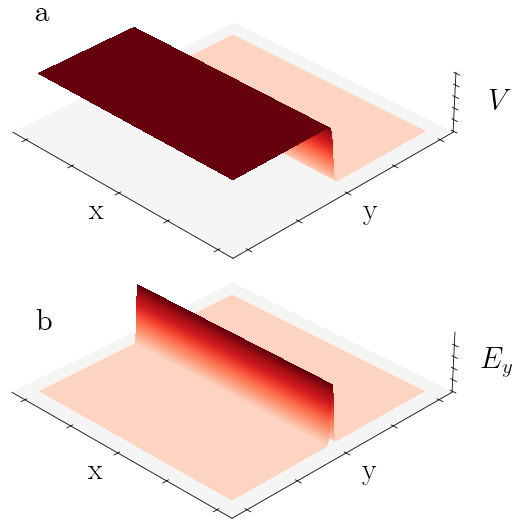
\includegraphics[width = 0.9\textwidth]{crosshair_marker/figures/gauge_trans.png}
    \caption{\label{fig:fields} \textbf{(a)} The electric potential used to generate our electric field. \textbf{(b)} The electric field, with only the nonzero $y$-component is shown.
    }
\end{figure}

Since we plan to calculate the response of the system under an applied electric field, let us start by precisely defining the potential we wish to apply to our system, and describing the effect on the Hamiltonian.

We wish to model the effect of raising the potential of one half of the system with respect to the other, resulting in an electric field across the boundary separating the two regions. Without loss of generality, let us consider raising the potential of the region below a dividing line at position $y = R_y$ with respect to the region above the line. In the continuum, this corresponds to an electric potential of the form $V(\textbf r) = -V_0 \theta(y - R_y) $, where $\theta$ is a Heaviside step function. The electric field acts over the line at $y = R_y$, as shown in figure \ref{fig:fields},
\begin{align}
    \textbf E(\textbf r)= V_0 \delta(y -R_y) \textbf e_y,
\end{align}
where $\textbf e_y$ is a unit vector in the $y$ direction. We transform to a gauge with zero scalar potential, representing the electric field with a magnetic vector potential,
\begin{align}
    \textbf A(\textbf r, t) = -V_0 t \delta(y - R_y) \textbf e_y.
\end{align}
Making the assumption that $V_0$ is small, we shall use Peierls substitution to describe the effect of a slow-varying magnetic vector potential on our lattice system~\cite{peierls_zur_1933}. The translation operators are modified by a Peierls phase $\ket{\textbf r_j}\bra{\textbf r_i} \rightarrow \ket{\textbf r_j}\bra{\textbf r_i} e^{i\alpha(\textbf r_i, \textbf r_j)}$, given by 
\begin{align}
    \alpha(\textbf r_i, \textbf r_j) = \int_{\textbf r_j}^{\textbf r_i} \textbf A(\textbf r) \cdot d\textbf r.
\end{align}
Note that we work in natural units, setting the electronic charge $q = \hbar = 1$. Given the form of the magnetic vector potential, we can see that translation operators only pick up a phase if they cross the line $y = R_y$. This is illustrated in fig.~\ref{fig:phase_lines_and_current}a. The Peierls phase can be expressed as
\begin{align}\label{eqn:phase}
    \alpha(\textbf r_i, \textbf r_j) = A(t) \left [ \theta( y_{i} - R_y) - \theta( y_{j} - R_y) \right ],
\end{align}
with $A(t) = V_0 t$. Thus, the Hamiltonian is modified according to
\begin{align}\label{eqn:H_shift}
    H(A) = e^{i A(t) \vartheta_{R_y}} H e^{-i A(t) \vartheta_{R_y}},
\end{align}
In the limit of small $A$, this can be expanded to first order,
\begin{align}\label{eqn:H_A_first_order}
    H(A) = H - i A(t) \left [ H, \vartheta_{R_y} \right ].
\end{align}
As we shall see in the next section, the change in the Hamiltonian is expressed in terms of a current operator for flow across the line $y = R_y$.

Note that for a static $A(t)$ in open boundaries, the $A$-dependence can be completely removed by a gauge transformation, so there will be no physical effect on our system. This is reflected by the fact that $\textbf E$ depends on $\partial_t A$, so static $A$ corresponds to zero electric field.
\begin{figure} 
    \begin{center}
        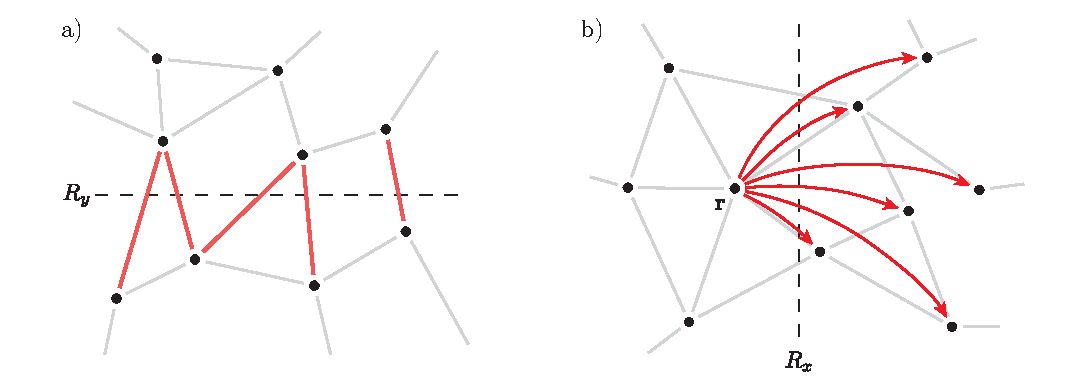
\includegraphics[width=0.9\textwidth]{crosshair_marker/figures/current_and_e_field.pdf}
        \caption{\textbf{(a)} A section of amorphous lattice is shown. All hopping terms in the Hamiltonian that cross the line $y = R_y$ acquire a Peierls phase given by eqn.~\ref{eqn:phase}, these are depicted in red. Unaffected hopping terms are shown in grey. Note that the phase is ill-defined when a site $\textbf r_i$ lies on the line, however this can be remedied by infinitesimally shifting $R_y$. \textbf{(b)} A depiction of the `local' current operator $J_{R_x}(\textbf{r})$ that calculates the total hopping to or from the site at $\textbf r$ that crosses the boundary at $R_x$. Background lattice is shown in grey.
        }\label{fig:phase_lines_and_current}
    \end{center}
\end{figure}


\subsection{Current Operators}\label{sec:current}

We construct an operator representing the flow of particles across a line bisecting the system. Again, without loss of generality, we will look at the flow of particles in the $x$-direction, across the vertical boundary at $x = R_x$. The number operator for particles to the right of this line is given by $\vartheta_{R_x}$. The time-evolution for the number of particles in this region is $\partial_t \langle \vartheta_{R_x} \rangle = i \langle [H, \vartheta_{R_x}] \rangle$. Thus, we can identify the operator representing flow of particles across the boundary as
\begin{align}\label{eqn:non_resolved_current}
    J_{R_x} = i[H, \vartheta_{R_x}].
\end{align}
This allows us to re-express eqn.~\ref{eqn:H_A_first_order} in the familiar form $H(A) = H - A J_{R_y}$, where $A$ is defined in equations \ref{eqn:phase}.

The operator $J_{R_x}$ evaluates the overall flow across the whole system, however in the following discussion we wish to separate the bulk and edge contributions. Thus let us decompose this operator into a sum of terms local to some point at $\textbf r$, according to
\begin{align}\label{eqn:current_operator}
    J_{R_x}(\textbf r) = \frac{1}{2} \left (
    \delta_{\textbf r} J_{R_x} +
    J_{R_x} \delta_{\textbf r}  \right ),
\end{align}
with $\delta_{\textbf r} = \ket{\textbf r}\bra{\textbf r}$. The two terms evaluate the contributions to $J_{R_x}$ from hopping into site $\textbf r$, and from hopping out of site $\textbf r$ respectively, a diagram is shown in fig.~\ref{fig:phase_lines_and_current}b. The factor of $1/2$ is included to ensure that $\sum_{\textbf r}J_{R_x}(\textbf r) = J_{R_x}$, since every pair of sites is counted twice. This decomposition is not unique --  there are many ways one could express $J_{R_x}$ as a sum over local terms. However, the final result will be insensitive to particular method since we shall sum over all the bulk contributions, which will be well-separated from edge contributions.

\subsection{Kato Dynamics}\label{sec:kato}
We will work in the adiabatic limit, with a Hamiltonian that changes over a long timescale $T$, where the local density of states in the bulk has an energy gap $\Delta$. We define the projector onto the occupied states at $t = 0$ as $P_0 = \sum_{\textup{occ}}\ket{\psi_i(0)} \bra{\psi_i(0)}$, where $\ket{\psi_i(0)}$ is an eigenstate of $H$ at $t = 0$. In general, time-evolution will result in a final state $P(t)$ that is related to the initial state by the Schr\"odinger equation. However. if the evolution is sufficiently slow (for $T\gg \Delta^{-1}$), we expect that $P_0$ will adiabatically evolve to the instantaneous projector, $P_{I}(t) =\sum_{\textup{band}}\ket{\psi_i(t)} \bra{\psi_i(t)} $, where $\ket{\psi_i(t)}$ are eigenstates of $H$ at time $t$~\cite{avron_adiabatic_1987}. To ensure that our time-evolution is exactly adiabatic, we use a formalism based on that introduced in~\cite{kato_adiabatic_1950}, although a modern description can be found in~\cite{simon_tosio_2018,avron_adiabatic_1987,avron_adiabatic_1999}. We sketch out the basics here. However for a detailed discussion, see appendix \ref{sec:kato_appendix}. 

Rather than using $H$ to generate time evolution, we define an adiabatic Hamiltonian, $K$, which satisfies the instantaneous Von-Neumann equation
\begin{align}\label{eqn:P_adiabatic_derivative}
    \partial_t P_I(t) = -i[K, P_I],
\end{align}
where the change in $P_I$ follows the instantaneous eigenstates of $H$. Using the identity $P \dot P P = 0$ (where dot denotes a time-derivative), we can verify that the equation is satisfied by $K$ of the form
\begin{align}\label{eqn:k_def}
    K(t) = i[\dot P_I , P_I].
\end{align}

The full time evolution of the projector follows the instantaneous eigenstates in the limit of large $T \gg \Delta$. Thus, in the following discussion, where we are working in the adiabatic regime, we may use eqn.~\ref{eqn:P_adiabatic_derivative} to describe the change in $P$, and drop the subscript on $P_I$, since all our time evolution is adiabatic. Having defined the adiabatic Hamiltonian, let us examine the exact form of $K$ for our applied electric field, as well as deriving an adiabatic equivalent of the current operator in eqn.~\ref{eqn:current_operator}.

\subsubsection{Adiabatic EM Fields}\label{sec:kato_field}

The time-dependence of our Hamiltonian is given by eqn.~\ref{eqn:H_shift}. We work in open boundaries, so the operator $e^{i A(t) \vartheta_{R_y}}$ behaves as a straightforward unitary rotation on the eigenstates. Note that in periodic boundaries, this operator would enforce twisted boundary conditions, shifting both the eigenstates and eigenenergies of $H$. Thus, the time-dependence of the projector is
\begin{align}
    P(t) = e^{i A(t) \vartheta_{R_y}} P_0 e^{-i A(t) \vartheta_{R_y}},
\end{align}
and the time-derivative is $\dot P =  i \dot A \left [ \vartheta_{R_y} , P \right ]$. This can be inserted into definition \ref{eqn:k_def} to arrive at the form of the adiabatic Hamiltonian,
\begin{align}\label{eqn:exact_k}
    K = \dot A \left ( P\vartheta_{R_y} Q +
    Q\vartheta_{R_y} P \right ),
\end{align}
where $Q = \1-P$ is the complement of the projector.

\subsubsection{Adiabatic Current}\label{sec:kato_current}

The adiabatic current operator is derived following an analogous argument to that in \textsection \ref{sec:current}. We find the change in particle number for the region $x>R_x$, given by $\vartheta_{R_x}$. In this case, however, we use the adiabatic Von-Neumann equation~\ref{eqn:P_adiabatic_derivative} to express the expectation value, $\partial_t \langle \vartheta_{R_x} \rangle = i \langle [K, \vartheta_{R_x}] \rangle$. Thus, we can identify an adiabatic current operator 
\begin{align}
    J_{R_x}^A = i [K,\vartheta_{R_x}].
\end{align}
As before, we can localise this operator to extract only the current hopping to and from a position $\textbf r$ according to 
\begin{align}\label{eqn:local_adiabatic_current}
    J^A_{R_x} (\textbf r) = \frac{1}{2} \{\delta_{\textbf r}, J_{R_x}^A \}.
\end{align}
In appendix \ref{sec:near_adiabatic} we discuss carefully how the non-adiabatic expression for current relates to the adiabatic form as we approach the adiabatic limit.

\subsection{Marker Derivation}\label{sec:marker_derivation}

Before we give the formal derivation, let us describe the physical intuition behind our topological marker, which can be understood as a localised version of the Hall conductivity. The standard Hall conductivity is measured by applying a uniform electric field to a 2D material and measuring the current induced perpendicular to the field. This current is quantised and corresponds to the Chern number of the Hamiltonian~\cite{laughlin_quantized_1981}. A disadvantage of this calculation is that it is necessarily global, with the electric field uniform over the system and the current measured across the whole sample. In a material with disorder or compound structure, the calculation gives no spatially-resolved information about its topological properties.

Our objective is to find an analogous quantity that can be spatially resolved, giving information about which parts of a complex material are responsible for topological behaviour. It is not obvious how one should localise the Hall conductivity: neither the electric field, nor the current operator can be easily localised to a point. Maxwell's laws prohibit one from creating an electric field at a single point only. Equally, on the lattice, it is difficult to write down a consistent expression for current at a point.

Despite that fact that neither electric field nor current can individually be made local to a point, it is possible to localise the overall Hall conductance. This is because both field and current can be localised to a line. By partitioning the system, and raising the electric potential of one part, we induce an electric field acting across the dividing line. Similarly, given a partition, by measuring the transfer of electrons from one part to the other, we are able to determine the current across the dividing line.


\begin{figure} [t]
    \begin{center}
        \resizebox{0.45\columnwidth}{!}{\input{crosshair_marker/tikzfigures/hall_diagram}}
        \caption{A schematic for local Hall measurement. The bottom half of the system has its potential raised with respect to the top half, generating an electric field acting over the horizontal line. Current is measured between the left and right halves, across the vertical line. The flow of charge is represented in blue, showing the curved path due to the presence of a magnetic field. The red shading shows the region around the crosshair where a nonzero contribution to the marker is measured.}\label{fig:crosshair_quarters}
    \end{center}
\end{figure}

The route to a local Hall current is to partition the system along two perpendicular dividing lines, as shown in fig.~\ref{fig:crosshair_quarters}. An electric field is induced between the top and bottom parts of the system by uniformly raising the voltage of the lower part. This will induce a vertical current acting across the dividing line. When the material has nonzero Chern number, a Hall current will also be induced from left to right. If the system is insulating (i.e.~gapped) we expect that all current should be localised to the region around the horizontal line. Measurement of the current is then taken over the vertical line, catching only induced current in the horizontal direction - effectively only the Hall current. We expect all nonzero contributions to come from the region around the point where the lines cross - motivating the name `crosshair marker'.

As we shall see in the following examples, this argument fails when the system becomes conducting and the gap closes. In a conducting system, current is no longer locally constrained - an electron can easily tunnel across the entire system. Thus we expect that the marker will be nonzero even very far from the crosshair. Consequently, as well as the central peak, we expect to see an additional term wherever conducting edge states are present, at any distance from the crosshair. 

We measure the local contribution to current across the line $x=R_x$ in the adiabatic regime. The current will be expressed in the form of a conductivity $J = \sigma E$, where $\sigma$ is to be determined. Our starting point is the expectation value of the current operator defined in \textsection\ref{sec:kato_current} for the case of a filled band of states,
\begin{align}
    \left \langle J^A_{R_x} (\textbf r) \right \rangle
    =\frac{1}{2}  \tr \left [P  \{\delta_{\textbf r}, J_{R_x}^A \} \right ],
\end{align}
where $P$ projects onto a fully occupied band of states. By cycling terms in the trace and using the identity $\1 = P+Q$, we can split this expression into two terms
\begin{align} \label{eqn:j_val}
\begin{aligned}
    \left \langle J^A_{R_x}(\textbf r) \right \rangle & = \tr_{\textbf r} 
    \left ( 
    P J_{R_x}^AP
    \right ) \\& +  
    \frac{1}{2}\tr_{\textbf r} 
    \left ( 
    P J_{R_x}^A Q + QJ_{R_x}^AP
    \right ),
\end{aligned}
\end{align}
where $\tr_{\textbf r} \vcentcolon= \tr(\delta_{\textbf r}\ ... )$ denotes a local trace over the internal degrees of freedom at site $\textbf r$. We treat these two terms separately. The first term is a local marker of Chern number whereas the second term vanishes. Considering only the second term, let us insert the exact form of $J_{R_x}^A = -[[\dot P,P], \vartheta_{R_x} ]$ and use the Jacobi identity,
\begin{align} \label{eqn:cyclic}
\begin{aligned}
    \tr _{\textbf r} \left ( P J_{R_x}^AQ  \right ) + h.c. &=
     \tr _{\textbf r} 
    \left ( P  
    \left [[P, \vartheta_{R_x}],\dot P\right ]
    Q  \right ) \\ 
    &+
     \tr _{\textbf r} 
    \left ( P  
    \left [[ \vartheta_{R_x},\dot P], P\right ]
    Q  \right )+ h.c.
\end{aligned}
\end{align}
Using the identities $P[P,\vartheta_{R_x}] =[P,\vartheta_{R_x}]Q $ and $P \dot P = \dot P Q$, we see that the first term here vanishes. We are left with the second term which can be written as
\begin{align}
    \tr _{\textbf r} \left ( P J_{R_x}Q  \right ) + h.c. = 
    - \tr _{\textbf r} 
    \left ( P  
    [ \vartheta_{R_x},\dot P]
    Q  \right )+ h.c.
\end{align}
Using $Q = \1-P$, we may re-express this in the form,
\begin{align}
    \tr _{\textbf r} \left ( P J_{R_x}Q  \right ) + h.c. = 
    - \tr _{\textbf r} 
    \left ( P  
    [ \vartheta_{R_x},\dot P]
    \right ) 
    + h.c.
\end{align}
Now, let us insert the exact form for $\dot P$ for a system undergoing adiabatic application of the step-function electric field defined in \textsection\ref{sec:kato_field}: $\dot P = i\dot A [\vartheta_{R_y} , P]$. We get a final expression
\begin{align}\label{eqn:constituent_vanish}
\begin{aligned}
    \tr _{\textbf r} \left ( P J_{R_x}Q  \right ) &+ h.c.\\ &=- i \dot A \tr _{\textbf r} 
    \left ( P  
    \left [ \vartheta_{R_x},[\vartheta_{R_y}, P]\right ]
    \right ) + h.c.
\end{aligned}
\end{align}
Writing out the terms in the trace explicitly, we get
\begin{align}
\begin{aligned}
    i\tr _{\textbf r} 
    \left ( P  
    \left [ \vartheta_{R_x},[\vartheta_{R_y}, P]\right ]
    \right ) &= i\tr_{\textbf{r}} (P\vartheta_{R_x}\vartheta_{R_y}P )\\
    &- i\tr_{\textbf{r}} (P\vartheta_{R_x}P\vartheta_{R_y})\\
    &- i\tr_{\textbf{r}} (\vartheta_{R_x}P\vartheta_{R_y}P)\\
    &+ i\tr_{\textbf{r}} (P\vartheta_{R_x}\vartheta_{R_y}).
\end{aligned}
\end{align}
The step functions commute with one another, and with $\delta_{\textbf r}$. This means that every constituent term in eqn.~\ref{eqn:constituent_vanish} is anti-Hermitian due to the factor of $i$. Thus the whole expression vanishes when the Hermitian conjugate is added, 
\begin{align}
    \tr _{\textbf r} \left ( P J_{R_x}Q  \right ) &+ h.c. = 0. 
\end{align}
Now, let us return to eqn \ref{eqn:j_val}. We have shown that the second term vanishes, so we are left with
\begin{align} 
    \left \langle J_{R_x}(\textbf r) \right \rangle & = \tr_{\textbf r} 
    \left ( 
    P J_{R_x}P
    \right )\\
    &=i \tr_{\textbf r} 
    \left ( 
    P [K, \vartheta_{R_x}] P
    \right ).
\end{align}
We use expression \ref{eqn:exact_k} to insert the exact form of $K$
\begin{align} 
    \left \langle J_{R_x}(\textbf r) \right \rangle & = i \dot A \tr_{\textbf r} 
    \left ( 
    P\vartheta_{R_x} Q \vartheta_{R_y} P
    \right ) + h.c.
\end{align}
Using the fact that $\dot A = -E$, we see that this expectation value has taken the form of a conductance, $\langle J \rangle = \sigma E$. We also use $Q = \1 - P$ to get the conductance in the form
\begin{align}\label{eqn:marker_form}
    \sigma(\textbf r; \textbf R) = 2 \Im \tr_{\textbf r} 
    \left ( 
    P\vartheta_{R_x} P \vartheta_{R_y} P
    \right ).
\end{align}

Finally we insert a factor of $2\pi$ to get the final expression for the marker
\begin{align}
    C(\textbf r;  \textbf R) = 4\pi \Im \tr_{\textbf r} 
    \left ( 
    P\vartheta_{R_x} P \vartheta_{R_y} P
    \right ).
\end{align}
This quantity is analogous to the Chern marker presented in appendix C of~\cite{kitaev_anyons_2006}, although where Kitaev used a global trace, here we have a local trace. Kitaev's marker was shown to exactly equal the Chern number in an infinite system. For finite system size, however, his marker vanishes due to edge-state contributions. By replacing the global trace with a local trace, we are here able to separate the bulk contribution from the edge contribution, allowing for the marker to be calculated in a finite system. We can extract the quantised Chern number by only summing over the bulk contributions -- found at $\textbf r$ close to $\textbf R$ -- and ignoring the edge-state terms at $\textbf r$ far from $\textbf R$.
We note two important caveats. Firstly the marker is only strictly well-defined as the sum of the bulk contributions around $\textbf R$, rather than as a function of $\textbf r$. This is because there is a degree of arbitrariness to how the current was made local to a point in definition \ref{eqn:current_operator}, since the purpose is to separate the bulk and edge contributions before summing only the bulk terms. Physically, the summed marker corresponds to the total current measured in the bulk over the line at $x = R_x$. 
The second caveat is that the adiabatic current defined in eqn.~\ref{eqn:local_adiabatic_current} only captures the current generated by the change in $P$ over time. However, it is also possible for a system to have persistent currents, i.e.~flow between occupied states that does not change the projector itself. Since this type of circulating current cannot change the number density at any site, it does not contribute to the net flow of electrons into a given region. Despite this, it can still contribute terms to the current defined in eqn.~\ref{eqn:current_operator}. Thus we must also require that the system has no persistent currents at any point in the adiabatic time evolution. This effect is explained in detail in appendix \ref{sec:near_adiabatic}.

Finally it is worth mentioning that -- following the argument presented for eqn.~\ref{eqn:chern_marker_from_kitaev} -- the crosshair marker can be used to calculate the Chern marker, $\mathfrak{C}$, given in~\cite{bianco_mapping_2011} according to
\begin{align}
    \mathfrak{C}(\textbf r) = \int d^2 \textbf R\ C(\textbf r;  \textbf R),
\end{align}
where the integral is over the whole system. 

